%!TEX program = xelatex
% 完整编译: xelatex -> bibtex -> xelatex -> xelatex
\documentclass[lang=cn,a4paper,cite=authoryear]{elegantpaper}
\songti

\title{\zihao{1}哈尔滨工业大学计算机科学与技术学院 \par 实验报告}
\date{}
% 本文档命令
\usepackage{array}
\usepackage{enumitem}
\usepackage{graphicx}
\usepackage{minted}
\usepackage{subfigure}
\newcommand{\ccr}[1]{\makecell{{\color{#1}\rule{1cm}{1cm}}}}

\begin{document}

\maketitle
\thispagestyle{empty}
\begin{center}
	\zihao{3}
   	{ 课程名称:  机器学习}\\[.5cm]
    { 课程类型:   选修}\\[.5cm]
    { 实验题目:  逻辑回归}\\[.5cm]
	{ 学 号:  1190202110}\\[.5cm]
	{ 姓 名: 田雪洋}\\[.5cm]
    { \date{\zhtoday}}\\[.50cm]
\end{center}


\newpage
\zihao{4}
\section*{\zihao{2}{一、实验目的}}
理解逻辑回归模型,掌握逻辑回归模型的参数估计算法。

\section*{\zihao{2}{二、实验要求及实验环境}}
\subsection*{\zihao{-2}{1.实验要求}}
实现两种损失函数的参数估计(1,无惩罚项;2.加入对参数的惩罚),可以采用梯度下降、共轭梯度或者牛顿法等。

\par 验证:1.可以手工生成两个分别类别数据(可以用高斯分布),验证你的算法。考察类条件分布不满足朴素贝叶斯假设,会得到什么样的结果。
\par 2. 逻辑回归有广泛的用处,例如广告预测。可以到UCI网站上,找一实际数据加以测试。


\subsection*{\zihao{-2}{2.实验环境}}
Windows10; python3.8.6;Pycharm 
\section*{\zihao{2}{三、设计思想(本程序中的用到的主要算法及数据结构)}}
对于给定的数据集$T=\left\{ \left( x_i,y_i \right) \right\} $,其中$x_i\epsilon R^n,y_i\epsilon \left\{ 0,1 \right\} $,可以使用logistics回归模型来进行分类。为此,我们对数据集进行如下规定:
$$
X=\left( \begin{matrix}
	x_1&		x_2&		\cdots&		x_n\\
\end{matrix} \right) ,y=\left[ \begin{array}{c}
	y_1\\
	y_2\\
	\vdots\\
	y_n\\
\end{array} \right] ,w^T=\left( \begin{matrix}
	w_1&		w_2&		\cdots&		w_n\\
\end{matrix} \right) 
$$
根据logistics回归模型,
\begin{equation}
P\left( y=1|x \right) =\frac{e^{wx}}{1+e^{wx}}=\pi \left( x \right) ,P\left( y=0|x \right) =\frac{1}{1+e^{wx}}=1-\pi \left( x \right) 
\end{equation}
则其似然函数为:
\begin{equation}
\prod_{i=1}^n{\left[ \pi \left( x_i \right) \right] ^{y_i}\left[ 1-\pi \left( x_i \right) \right] ^{1-y_i}}
\end{equation}
则其对数似然函数为:
\begin{equation}
L\left( W \right) =\sum_{i=1}^n{\left[ y_i\left( w\cdot x_i \right) -\log \left( 1+e^{w\cdot x_i} \right) \right]}
\end{equation}      
仿照实验1的结论,为了避免过拟合现象,我们在似然函数后添加正则项,得到:
\begin{equation}
L\left( W \right) =\sum_{i=1}^n{\left[ y_i\left( w\cdot x_i \right) -\log \left( 1+e^{w\cdot x_i} \right) \right]}+\frac{\lambda}{2}\left\| w \right\| ^2
\end{equation}
对$L\left( W \right)$求极大值,便可以得到$w$的估计值了。
在这里我们采用多种方法求解。
\subsection*{\zihao{-2}{1.梯度下降法}}
\par 首先我们使用梯度下降法来求解,为此,我们需要转换为求$-L\left( W \right)$的极小值。在综合考虑数据集的样本数量后,我们最终确定目标函数为:
\begin{equation}
	\mathop {arg\min} \limits_{w}-\frac{1}{n}L\left( W \right) 
\end{equation}    
则梯度下降法的迭代公式为:
\begin{equation}
	W=W-\eta \lambda W-\frac{\eta}{n}\frac{\partial L\left( W \right)}{\partial W}=W-\eta \lambda W+\frac{\eta}{n}\sum_{i=1}^n{\left( y_ix_i-\frac{x_i}{1+e^{w\cdot x_i}} \right)}	 
\end{equation}
其中$\eta \lambda W$为正则项。
\subsection*{\zihao{-2}{2.共轭梯度法}}
\par 此外,还可以使用共轭梯度法进行求解,由于共轭梯度法要求系数矩阵为对称矩阵且正定,但显然本题的一阶导方程不满足,因此,对于一般形式的线性方程,共轭梯度法需要求其Hessian矩阵。其迭代过程如下:
\begin{enumerate}[(1)]
	\item 初始条件
	      $$
	      \begin{gathered}
	      	g_{1}=H x_{1}-b \\
	      	d_{1}=r_{1}=-g_{1}
	      \end{gathered}
	      $$
	\item 迭代式
	$$
	\begin{gathered}
		a_{k}=\frac{d_{k}^{T} r_{k}}{d_{k}^{T} H d_{k}} \\
		x_{k+1}=x_{k}+a_{k} d_{k} \\
		r_{k+1}=r_{k}-a_{k} H d_{k} \\
		\beta_{k}=\frac{r_{k+1}^{T} H d_{k}}{d_{k}^{T} H d_{k}} \\
		d_{k+1}=r_{k+1}-\beta_{k} d_{k}
	\end{gathered}
	$$
所以只需要求解出似然函数的一阶导数的Hessian矩阵即可,Hessian矩阵$H=X^TAX$,其中,
$$
A=\left( \begin{matrix}
	\pi \left( x_1 \right) \left[ 1-\pi \left( x_1 \right) \right]&		0&		\cdots&		0\\
	0&		\pi \left( x_2 \right) \left[ 1-\pi \left( x_2 \right) \right]&		\cdots&		0\\
	\vdots&		\vdots&		\ddots&		\vdots\\
	0&		0&		\cdots&		\pi \left( x_n \right) \left[ 1-\pi \left( x_n \right) \right]\\
\end{matrix} \right) 
$$


\end{enumerate}
\subsection*{\zihao{-2}{3.牛顿法}}
牛顿法的基本思想是用梯度信息和二阶导数对目标函数进行逼近,然后把极小值作为新的迭代点,并不断重复这一过程,直到求出极小点。
其步骤可以总结为以下四步:
\begin{enumerate}[(1)]
	\item 设置初始点及终止条件
	\item 检验是否满足终止条件
	\item 计算二阶导数,并确定搜索方向
	$$
	d_{k}: \nabla^{2} f\left(x_{k}\right) d=-\nabla f\left(x_{k}\right)
	$$
	\item 计算下一个迭代点
	$$
	x_{k+1}=x_{k}+d_{k}
	$$
	重复步骤(2)
\end{enumerate}
本题的一阶导数在上文中已经给出,所以下面只需要求解二阶导数即可:
$$
\frac{\partial ^2L}{\partial \mathbf{w}\partial \mathbf{w}^{\mathbf{T}}}=\sum_{i=1}^n{\left( x_ix_{i}^{T}\frac{e^{w\cdot x_i}}{1+e^{w\cdot x_i}}\frac{1}{1+e^{w\cdot x_i}} \right)}
$$
则牛顿法的完整迭代式为:
$$
x_{k+1}=x_k-\alpha \left( \frac{\partial ^2L}{\partial \mathbf{w}\partial \mathbf{w}^{\mathbf{T}}}^{-1}\frac{\partial L\left( W \right)}{\partial W}+\lambda w \right) 
$$
\section*{\zihao{2}{四、实验结果与分析}}
\subsection*{\zihao{-2}{1.生成数据}}
首先,先产生若干符合高斯分布的样本点,其中反例均值为[-1, -0.3],正例均值为[0.8, 0.3],方差均为0.2,若不满足贝叶斯假设,则协方差为:0.1。训练集的样本点数为50,测试集的样本点数为100,学习速率为1,正则项系数为0.01,精度为$10^{-5}$。

\subsection*{\zihao{-2}{2.四次实验如下}}
\subsubsection*{\zihao{-3}{2.1.有惩罚项,满足贝叶斯假设}}
对于有惩罚项,满足贝叶斯假设的测试集和训练集,我们的到了如下结果:
\begin{itemize}
	\par
\item 梯度下降法
\begin{center}
	\begin{figure}[H]
		\centering
		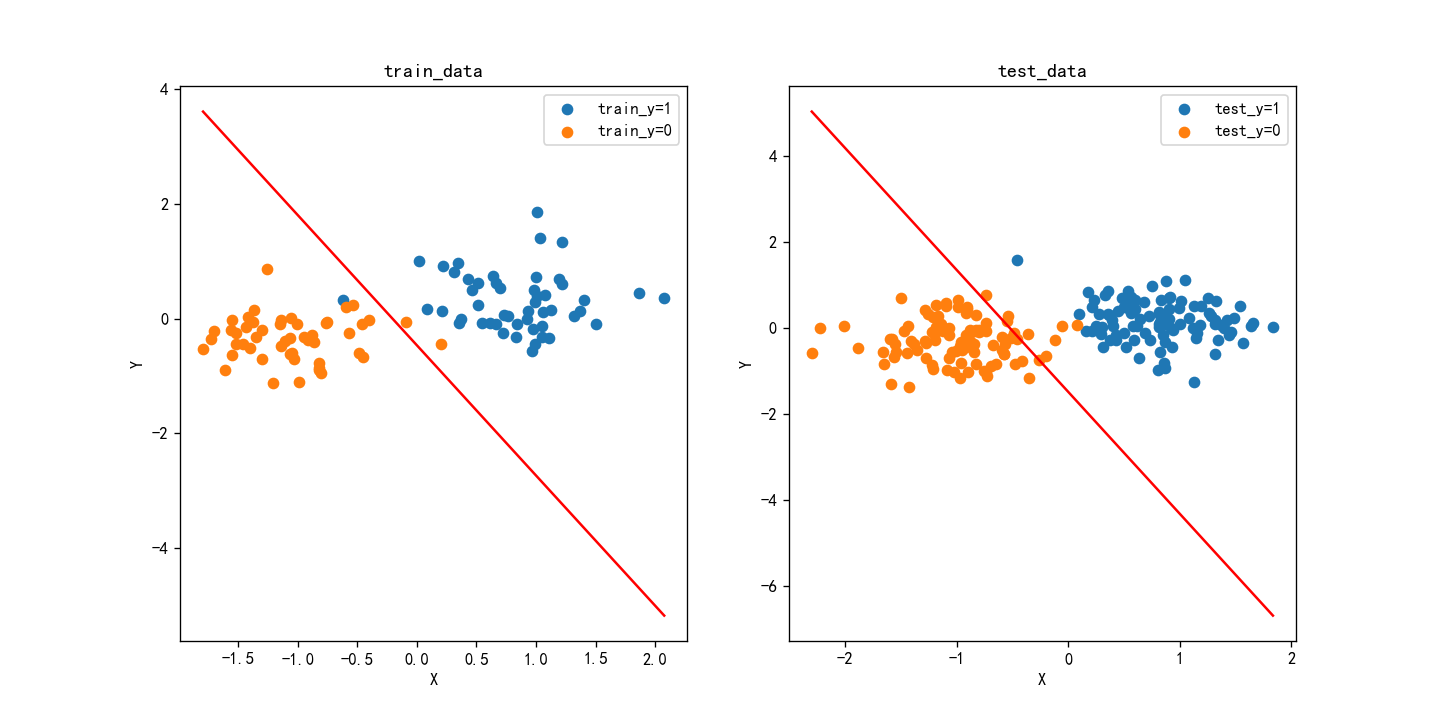
\includegraphics[scale=0.5]{test01}
	\end{figure}
\end{center}
其中训练集的准确率为:97\%,测试集的准确率为99\%。可以看到logistics回归在此时取到了较好的分类效果,可以明显地分开两个类。
\par
\item 牛顿法
\begin{center}
	\begin{figure}[H]
		\centering
		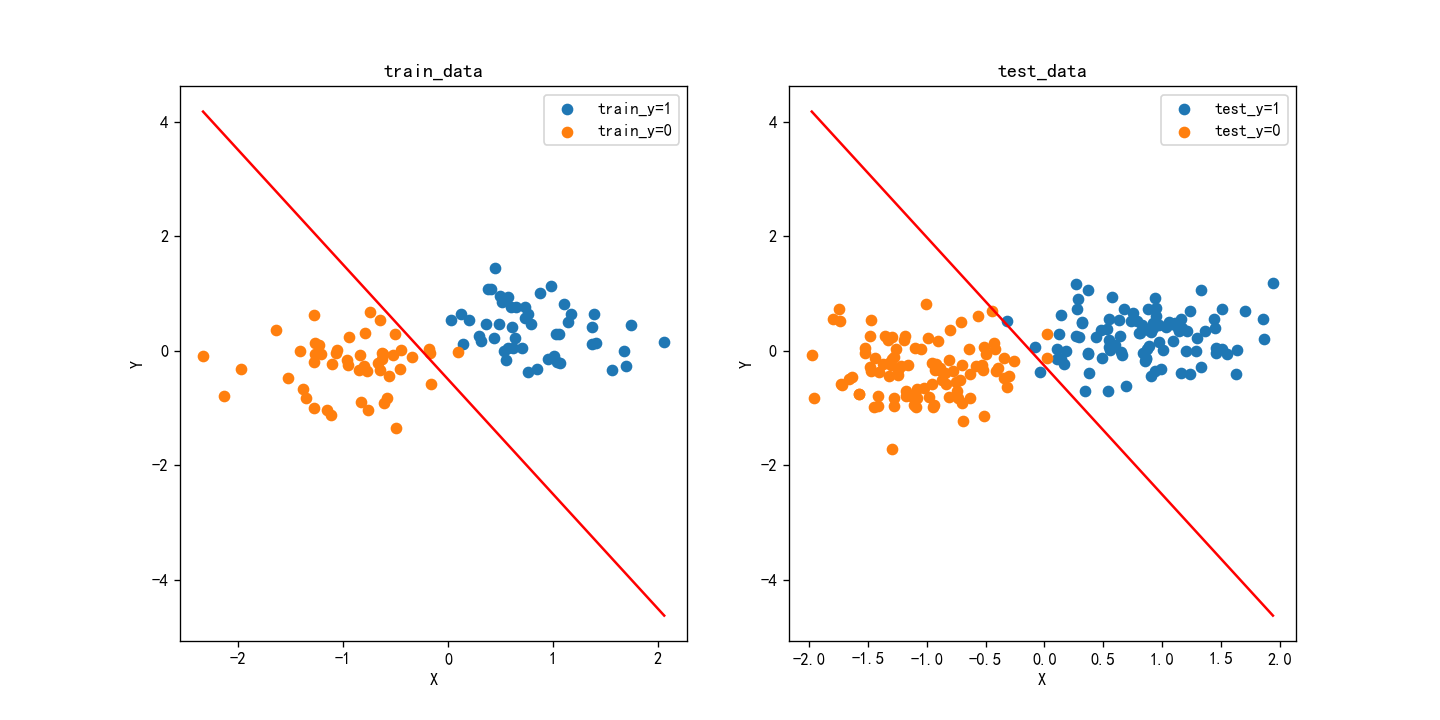
\includegraphics[scale=0.5]{nttest01}
	\end{figure}
\end{center}
其中训练集的准确率为:97\%,测试集的准确率为98.5\%。可以看到logistics回归在此时取到了较好的分类效果,可以明显地分开两个类。
\par
\item 共轭梯度法
\begin{center}
	\begin{figure}[H]
		\centering
		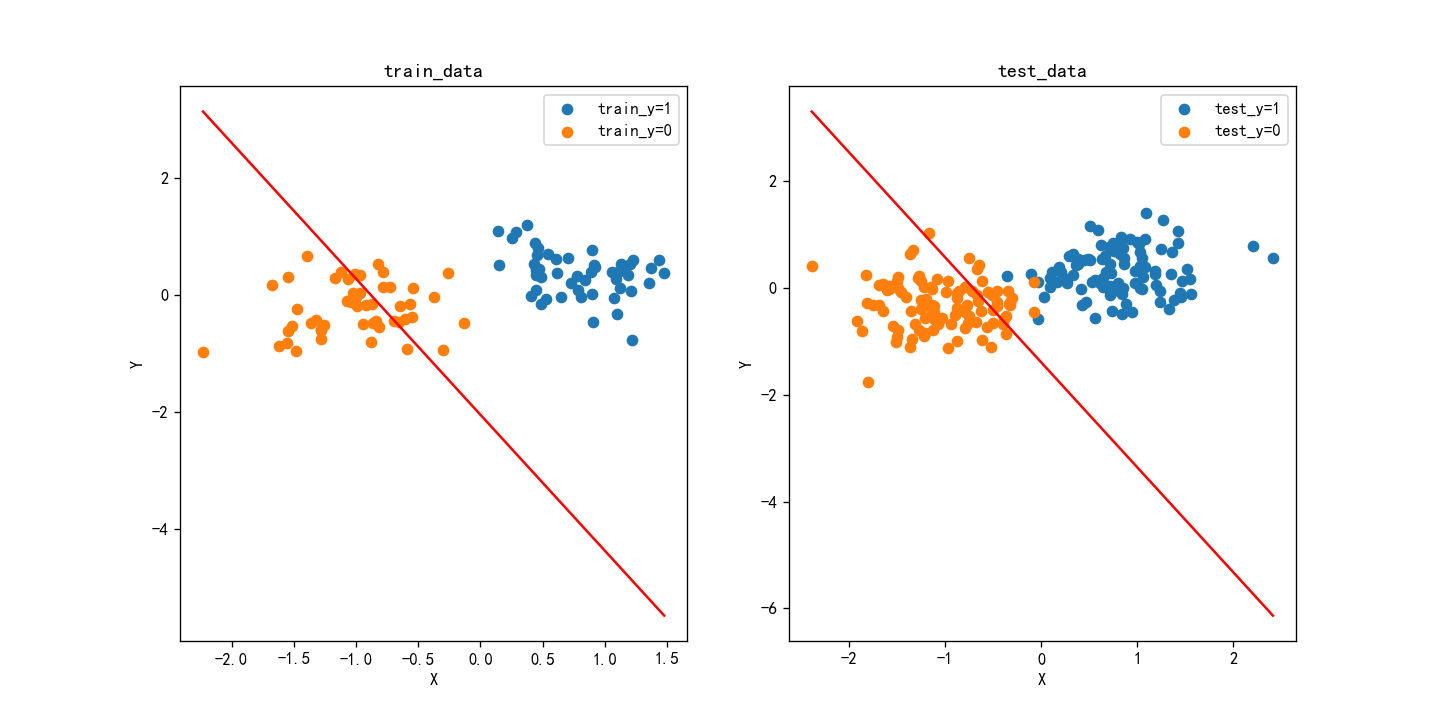
\includegraphics[scale=0.5]{gctest01}
	\end{figure}
\end{center}
其中训练集的准确率为:84\%,测试集的准确率为83\%。可以看到logistics回归在使用共轭梯度法时,取得的效果并不是很理想。
\end{itemize}
\subsubsection*{\zihao{-3}{2.2.有惩罚项,不满足贝叶斯假设}}
对于有惩罚项,不满足贝叶斯假设的测试集和训练集,我们的到了如下结果:
\begin{itemize}
	\par
	\item 梯度下降法
	\begin{center}
		\begin{figure}[H]
			\centering
			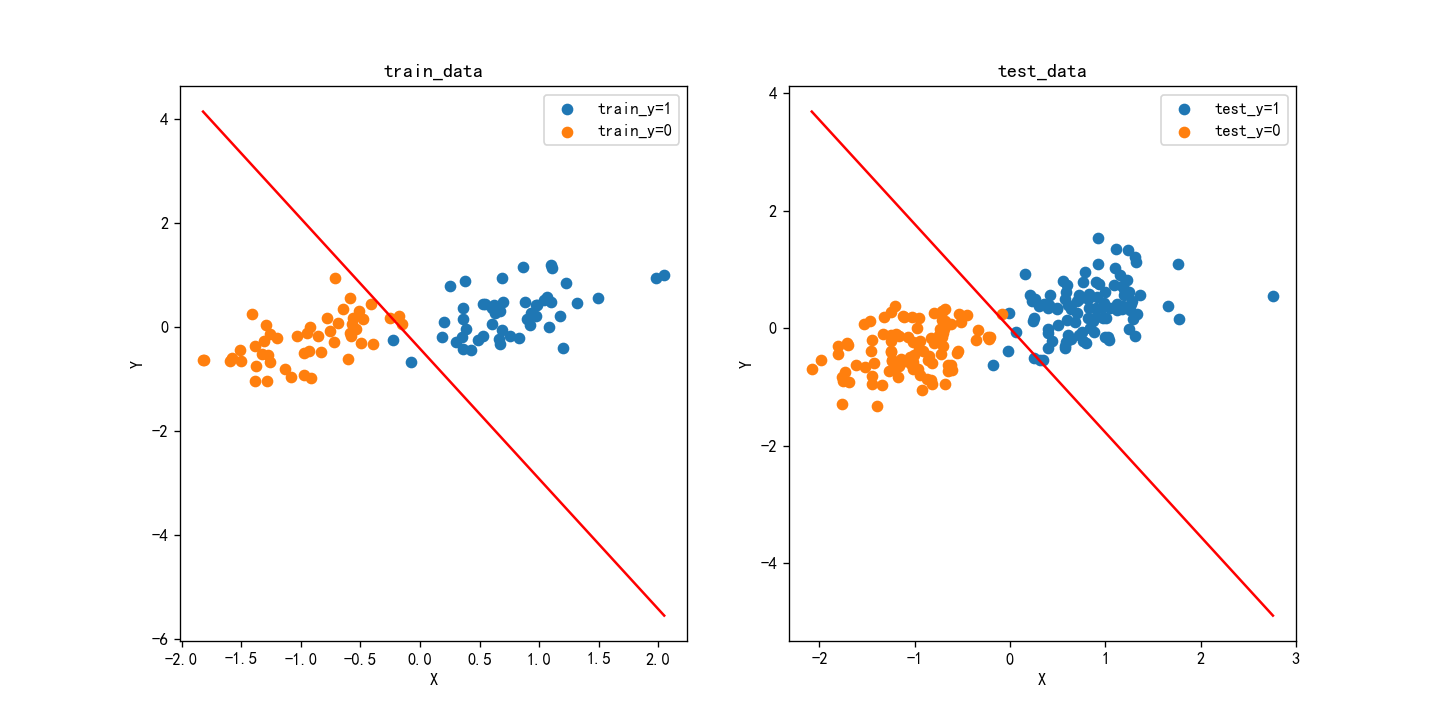
\includegraphics[scale=0.5]{test02}
		\end{figure}
	\end{center}
其中训练集的准确率为:96\%,测试集的准确率为98.5\%。可以看到logistics回归在此时取到了较好的分类效果,可以明显地分开两个类。
	\par
	\item 牛顿法
	\begin{center}
		\begin{figure}[H]
			\centering
			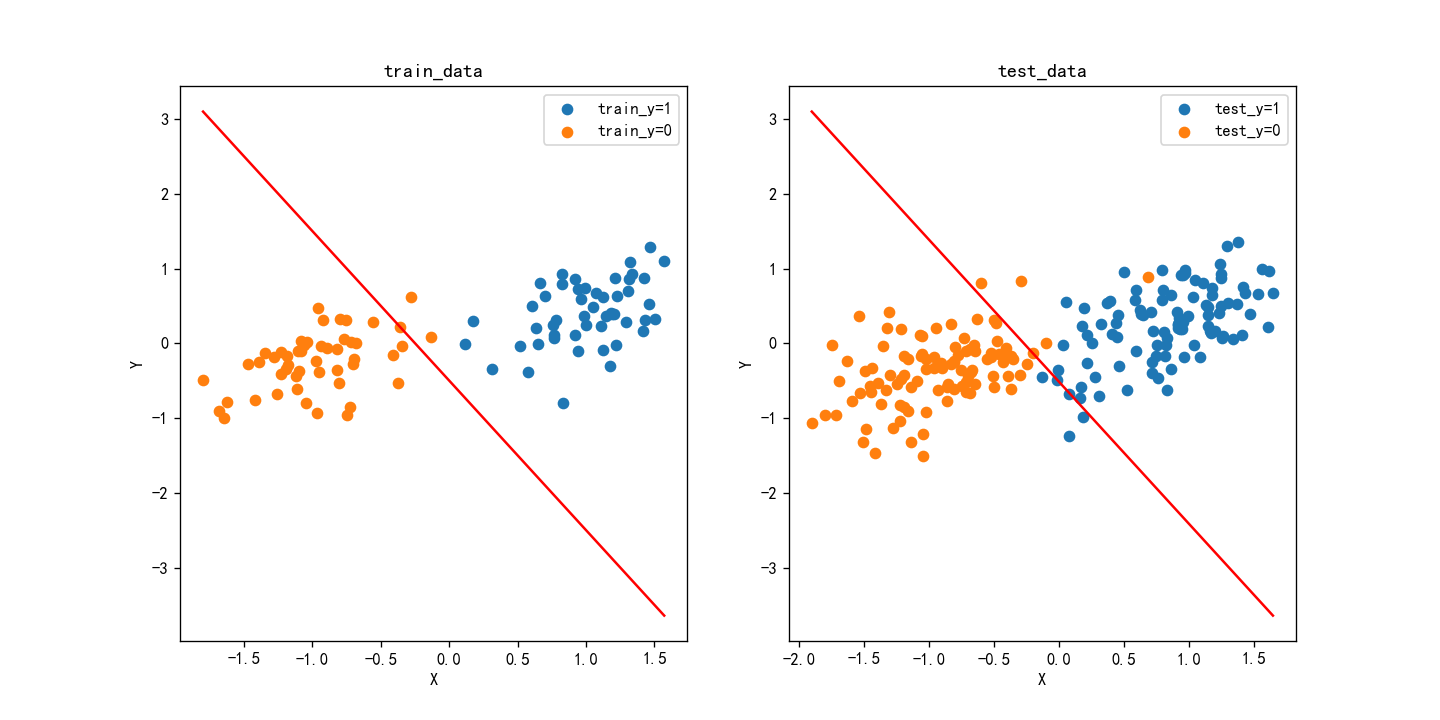
\includegraphics[scale=0.5]{nttest02}
		\end{figure}
	\end{center}
其中训练集的准确率为:98\%,测试集的准确率为95.5\%。可以看到logistics回归在此时取到了较好的分类效果,可以明显地分开两个类。
	\par
	\item 共轭梯度法
	\begin{center}
		\begin{figure}[H]
			\centering
			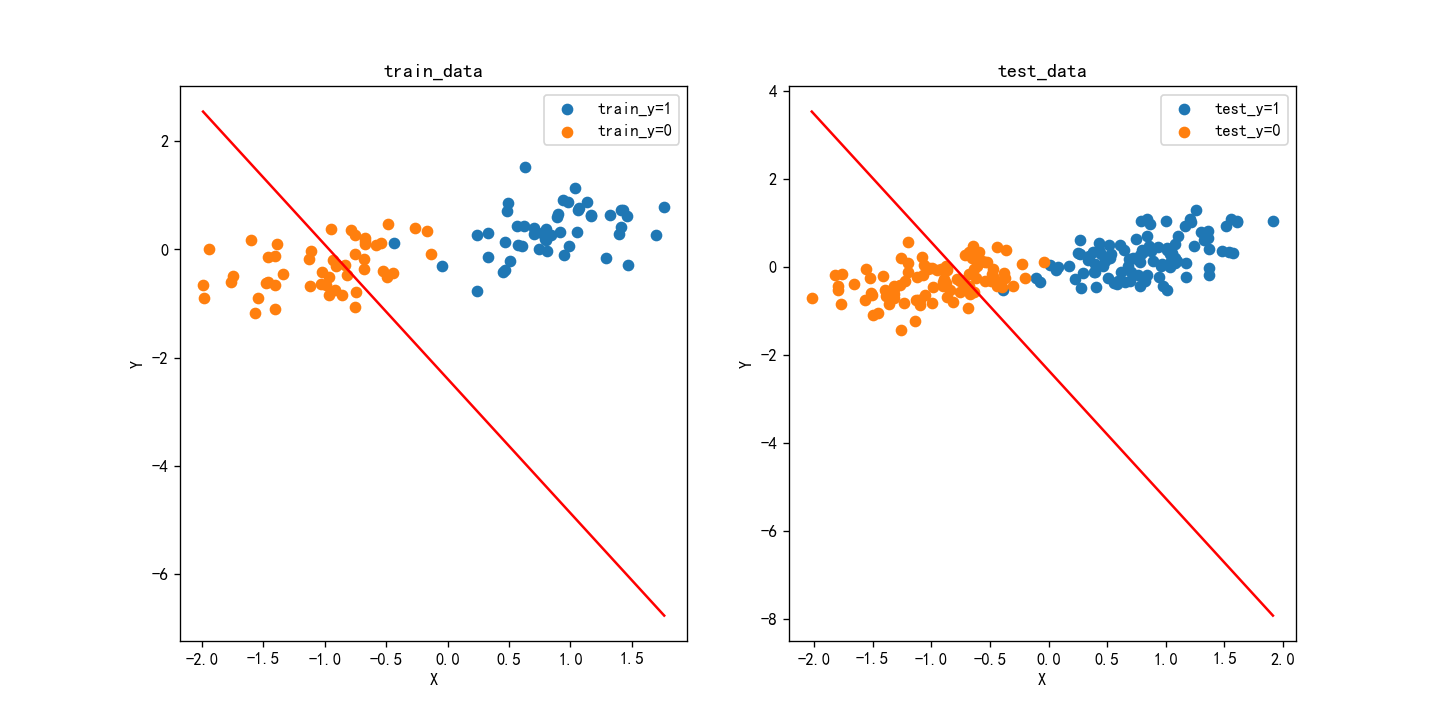
\includegraphics[scale=0.5]{gctest02}
		\end{figure}
	\end{center}
	其中训练集的准确率为:81\%,测试集的准确率为83.5\%。可以看到logistics回归在使用共轭梯度法时,取得的效果并不是很理想。
\end{itemize}
\subsubsection*{\zihao{-3}{2.3.无惩罚项,满足贝叶斯假设}}
对于无惩罚项,满足贝叶斯假设的测试集和训练集,我们的到了如下结果:
\begin{itemize}
	\par
	\item 梯度下降法
	\begin{center}
		\begin{figure}[H]
			\centering
			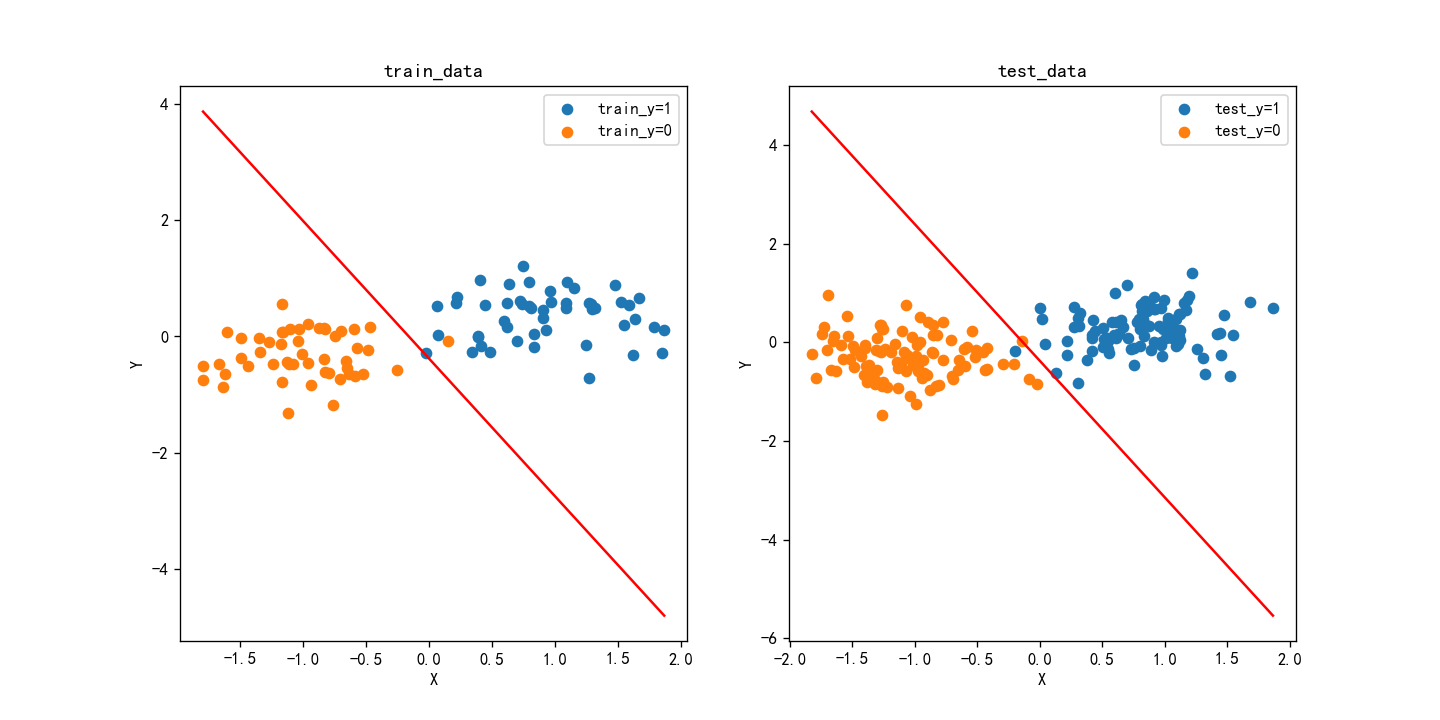
\includegraphics[scale=0.5]{test03}
		\end{figure}
	\end{center}
	其中训练集的准确率为:98\%,测试集的准确率为99\%。可以看到logistics回归在此时取到了较好的分类效果,可以明显地分开两个类。
	\par
	\item 牛顿法
	\begin{center}
		\begin{figure}[H]
			\centering
			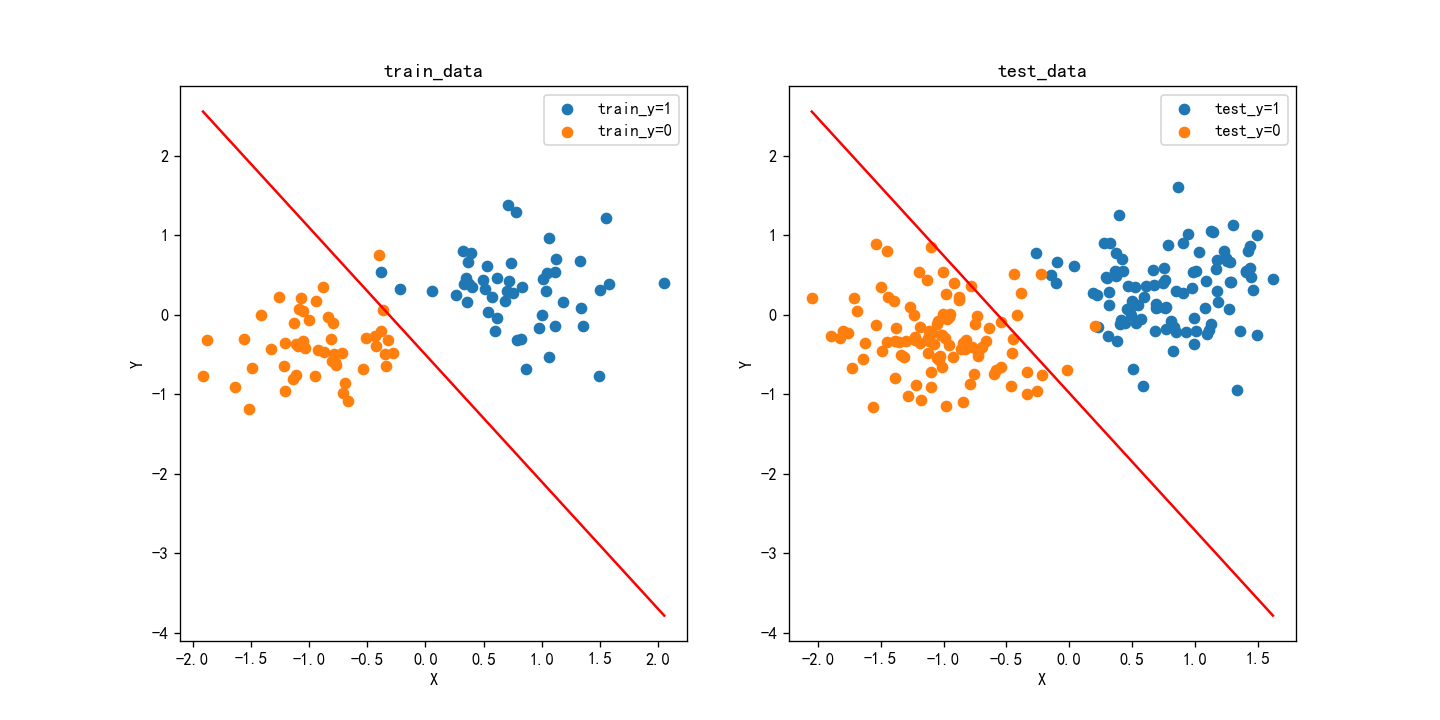
\includegraphics[scale=0.5]{nttest03}
		\end{figure}
	\end{center}
	其中训练集的准确率为:99\%,测试集的准确率为98\%。可以看到logistics回归在此时取到了较好的分类效果,可以明显地分开两个类。
	\par
	\item 共轭梯度法
	\begin{center}
		\begin{figure}[H]
			\centering
			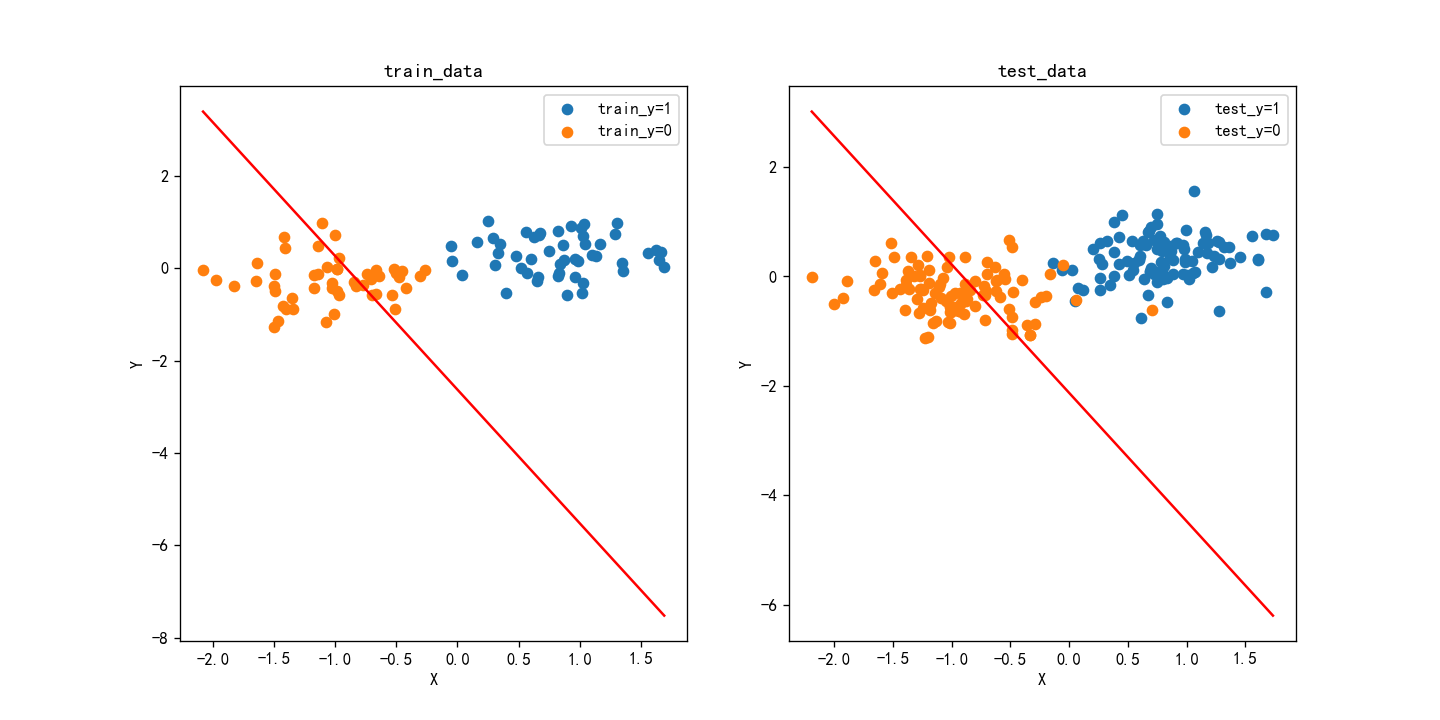
\includegraphics[scale=0.5]{gctest03}
		\end{figure}
	\end{center}
	其中训练集的准确率为:81\%,测试集的准确率为85\%。可以看到logistics回归在使用共轭梯度法时,取得的效果并不是很理想。
\end{itemize}
\subsubsection*{\zihao{-3}{2.4.无惩罚项,不满足贝叶斯假设}}
对于无惩罚项,不满足贝叶斯假设的测试集和训练集,我们的到了如下结果:
\begin{itemize}
	\par
	\item 梯度下降法
	\begin{center}
		\begin{figure}[H]
			\centering
			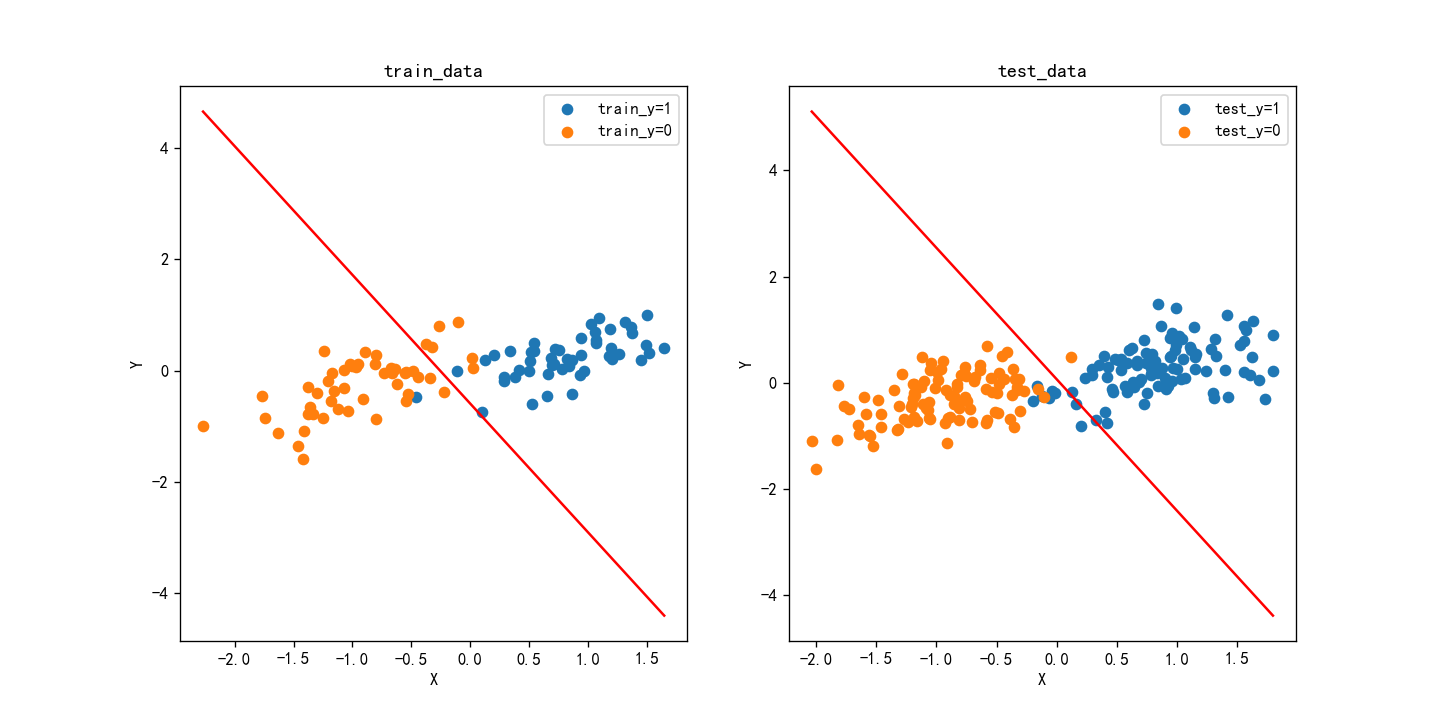
\includegraphics[scale=0.5]{test04}
		\end{figure}
	\end{center}
	其中训练集的准确率为:93\%,测试集的准确率为97.5\%。可以看到logistics回归在此时取到了较好的分类效果,可以明显地分开两个类。
	\par
	\item 牛顿法
	\begin{center}
		\begin{figure}[H]
			\centering
			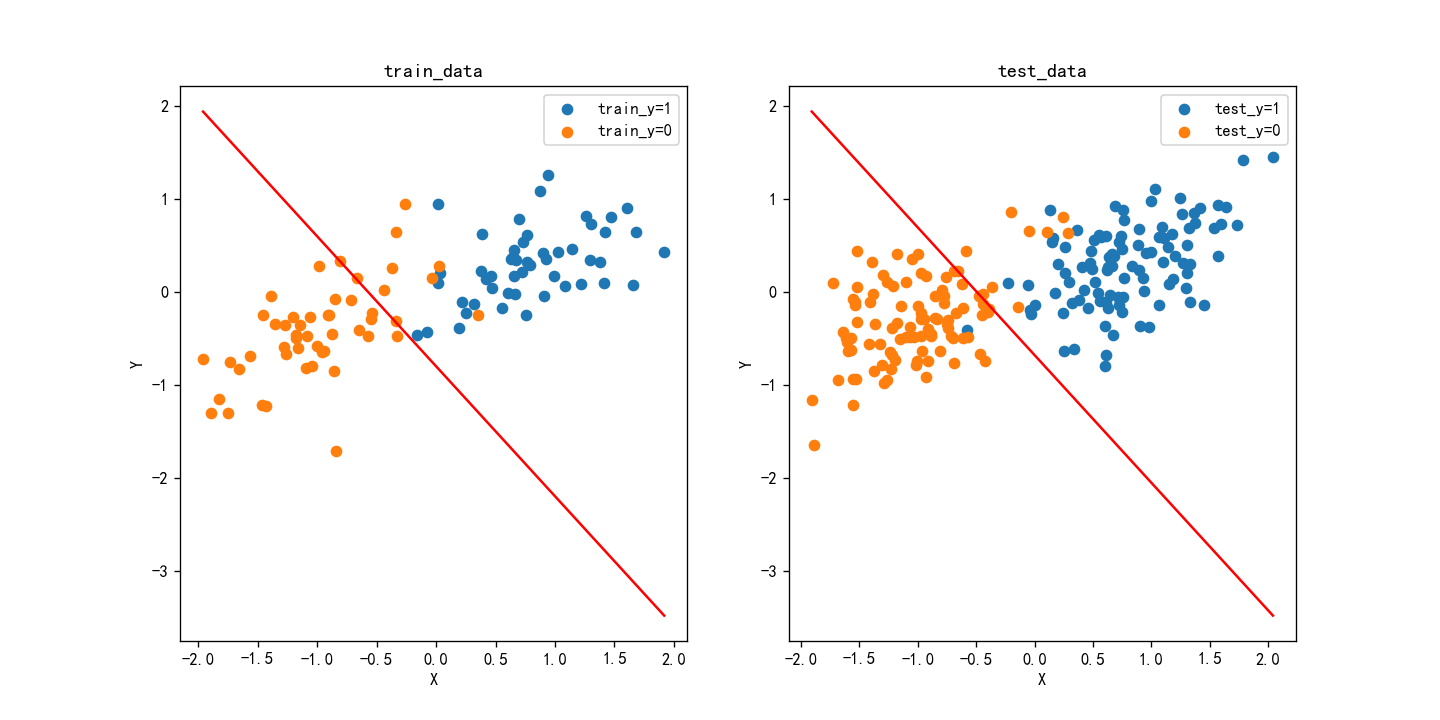
\includegraphics[scale=0.5]{nttest04}
		\end{figure}
	\end{center}
	其中训练集的准确率为:90\%,测试集的准确率为91.5\%。可以看到logistics回归在此时取到了较好的分类效果,可以明显地分开两个类。
	\par
	\item 共轭梯度法
	\begin{center}
		\begin{figure}[H]
			\centering
			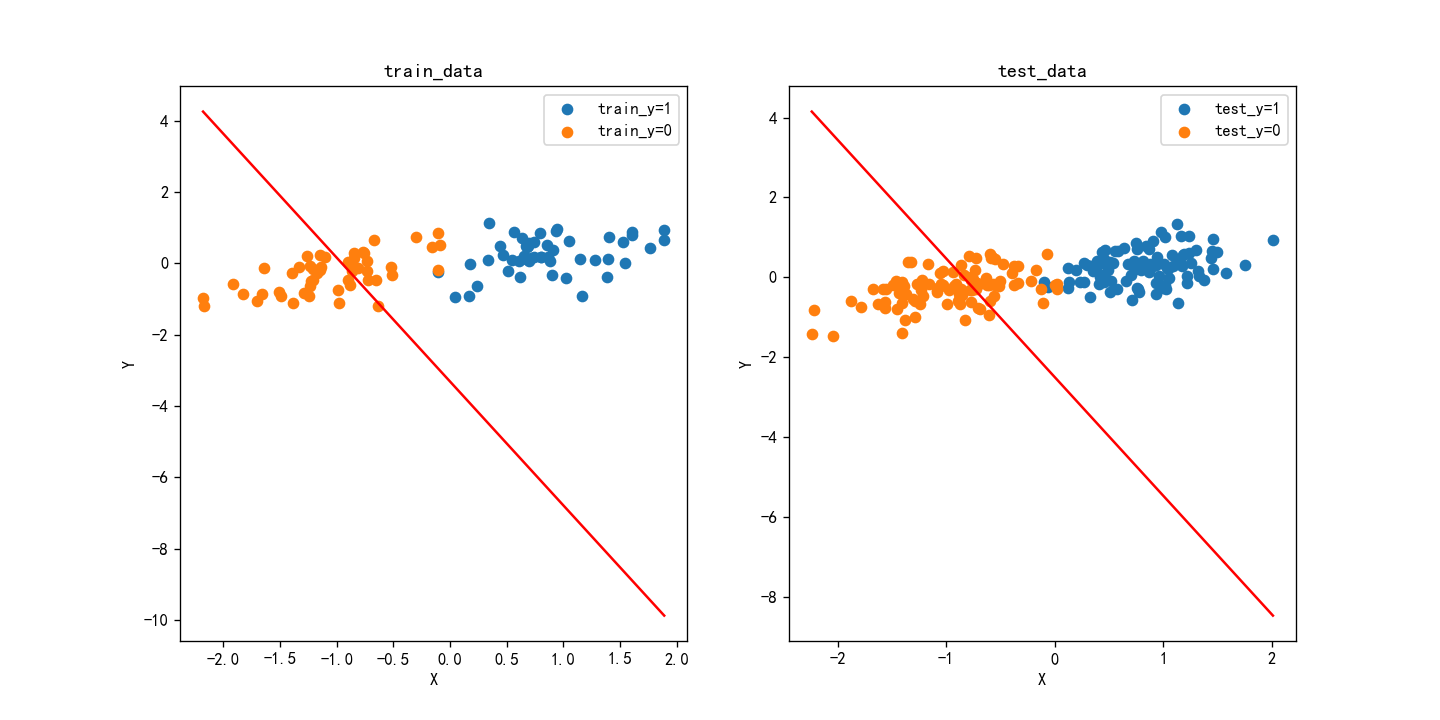
\includegraphics[scale=0.5]{gctest04}
		\end{figure}
	\end{center}
	其中训练集的准确率为:85\%,测试集的准确率为84\%。可以看到logistics回归在使用共轭梯度法时,取得的效果并不是很理想。
\end{itemize}
\subsection*{\zihao{-2}{3.UCI数据集}}
UCI数据集中的breast\_cancer数据集是简单经典的用于二分类任务的数据集。本次实验采用乳腺癌数据集进行logistics回归模型的测试。原数据集中有30个特征,样本数量为569。各个样本的特征如下:
\begin{center}
	\begin{figure}[H]
		\centering
		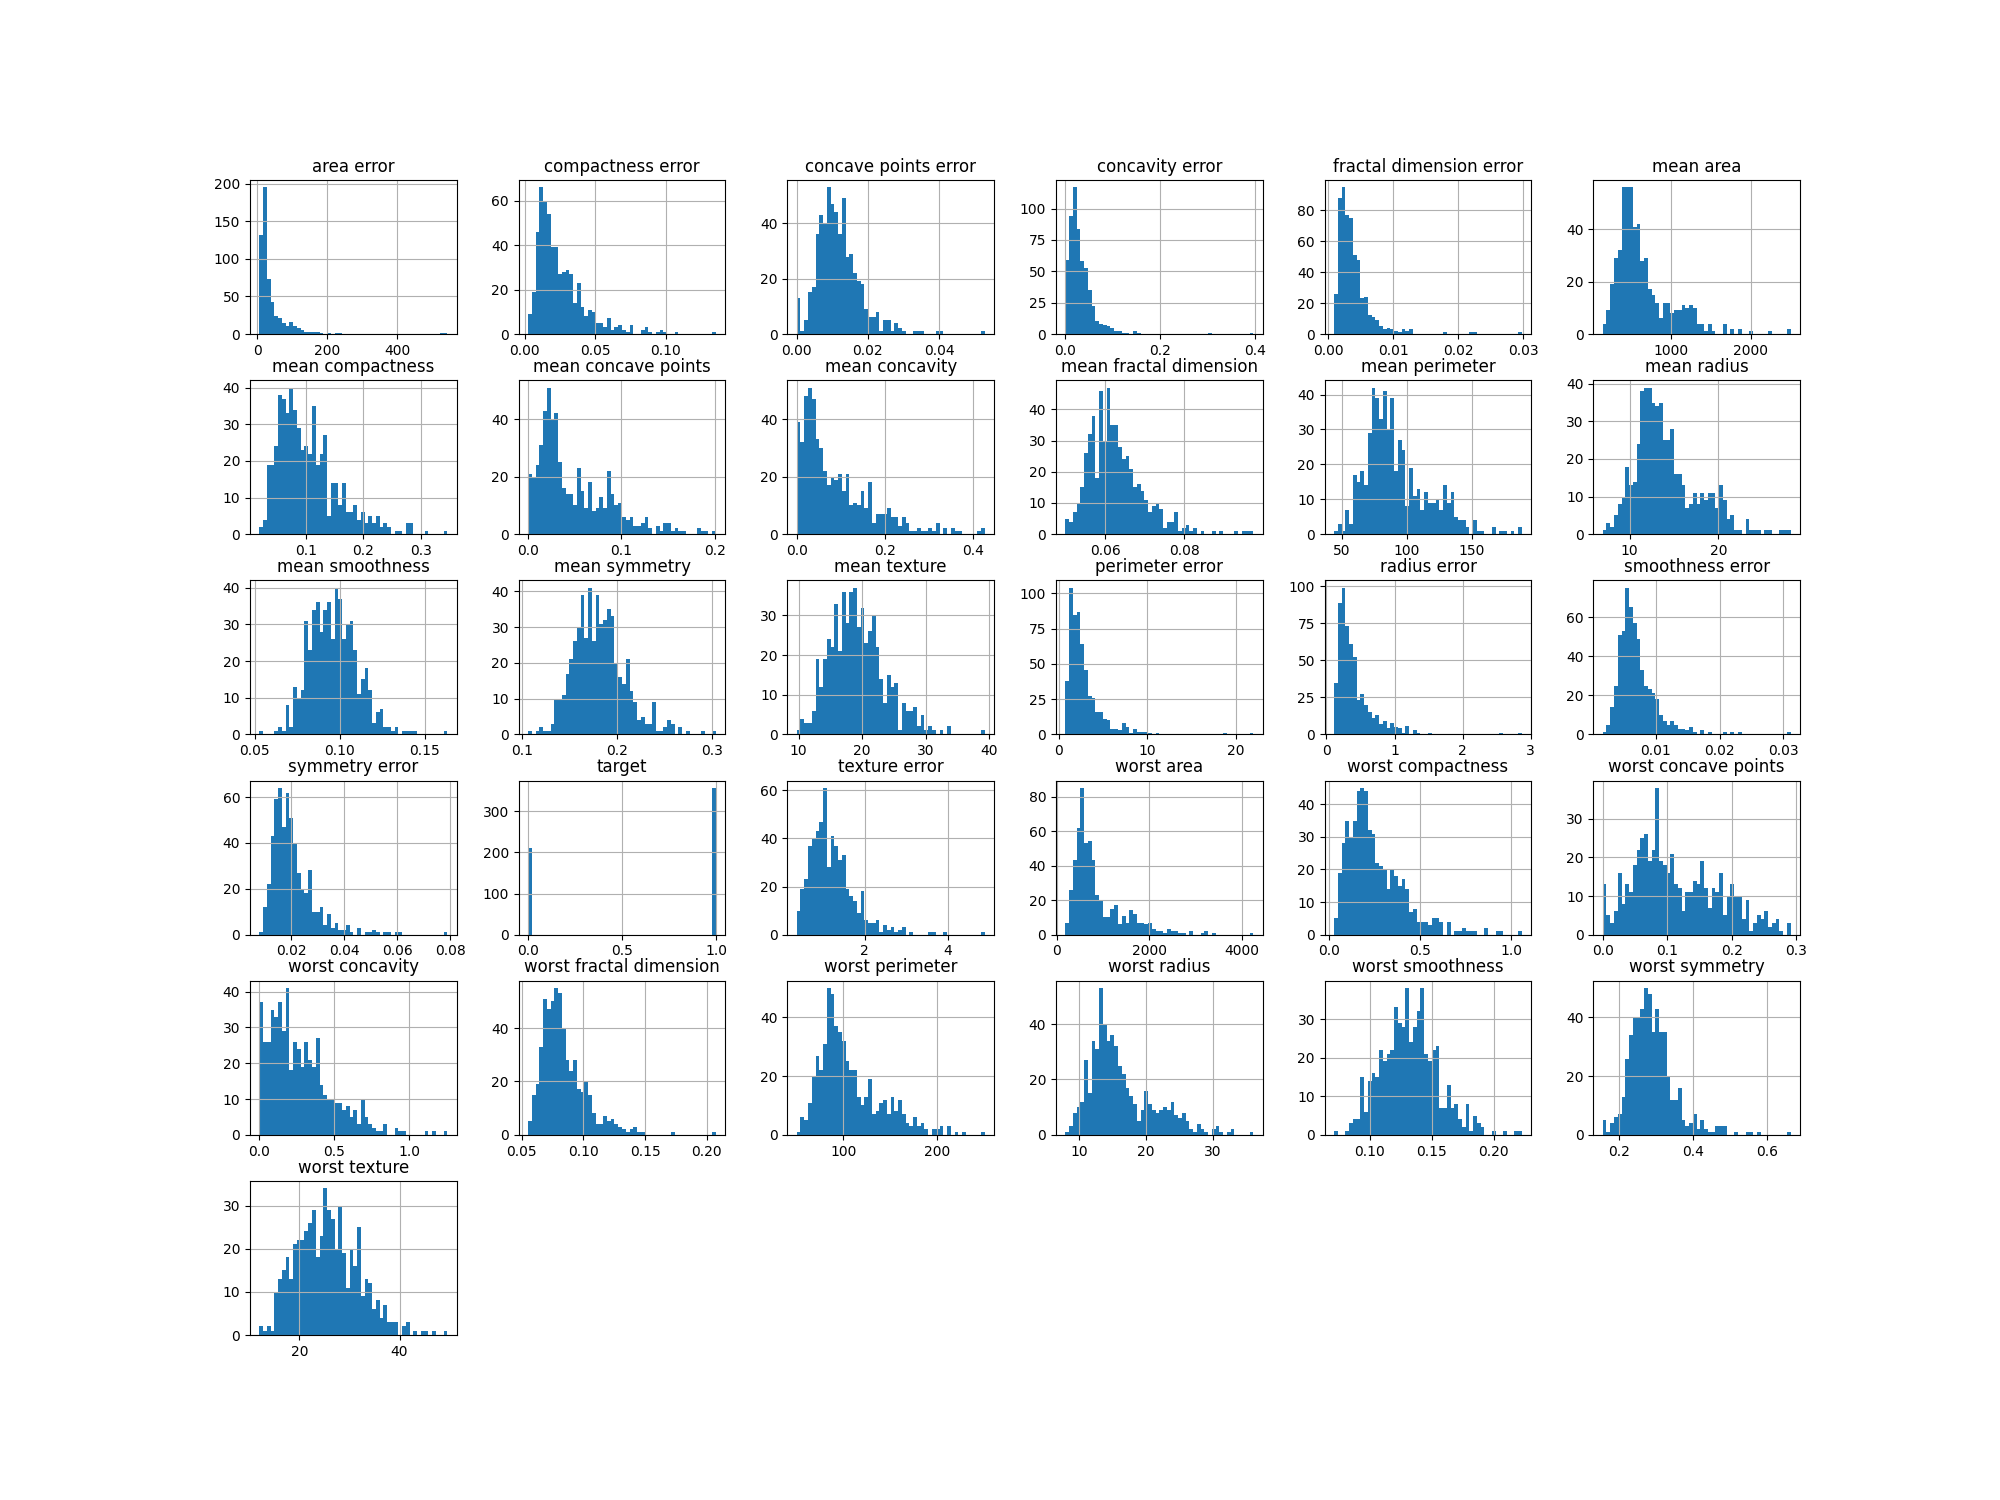
\includegraphics[scale=0.3]{fecter_analisy}
		\centering
	\end{figure}
\end{center}


在本次实验中,首先将数据进行归一化处理,然后代入模型进行测试,结果测试集中的准确率为:63.6\%,测试集的准确率为:61.4\%。可以看到无论是测试集还是训练集,模型的准确率都很低。经分析,主要原因是,我写的这个logistics模型只适用于线性可分的数据集,而本数据集是线性不可分的,因此训练出的效果极差。

\section*{\zihao{2}{五、结论}}
\begin{itemize}
\item  对于梯度下降法,和牛顿法,logistics回归的效果较好,但共轭梯度法的效果较差
\item  对于牛顿法,由于需要计算二阶导数(或黑塞矩阵)的逆,其收敛速度较慢,而且还可能不存在逆。
\item  从实验可以看出,当数据集满足朴素贝叶斯假设时logistics回归模型的分类表现略好于不满足朴素贝叶斯假设时的
\end{itemize}
\section*{\zihao{2}{六、参考文献}}
\begin{enumerate}[(1)]
\item  周志华 著. 机器学习, 北京: 清华大学出版社, 2016.1
\item  李航 著. 统计学习方法,北京:清华大学出版社,2020.6
\end{enumerate}
\section*{\zihao{2}{七、附录:源代码(带注释)}}
源代码见相关文件
\begin{enumerate}[(1)]
	\item  gd.py:数据预处理,生成,梯度下降法,牛顿法,共轭梯度法的logistics模型
	\item  test01.py-test04.py:梯度下降法在数据集是否满足贝叶斯假设,是否含正则项的求解过程及绘图
	\item  nt\_test01.py-nt\_test04.py:牛顿法在数据集是否满足贝叶斯假设,是否含正则项的求解过程及绘图
	\item  gc\_test01.py-gc\_test04.py:共轭梯度法在数据集是否满足贝叶斯假设,是否含正则项的求解过程及绘图
	\item  cancer.py 乳腺癌数据集进行logistics回归模型的测试及绘图
\end{enumerate}
\end{document}